
%% bare_conf.tex
%% V1.3
%% 2007/01/11
%% by Michael Shell
%% See:
%% http://www.michaelshell.org/
%% for current contact information.
%%
%% This is a skeleton file demonstrating the use of IEEEtran.cls
%% (requires IEEEtran.cls version 1.7 or later) with an IEEE conference paper.
%%
%% Support sites:
%% http://www.michaelshell.org/tex/ieeetran/
%% http://www.ctan.org/tex-archive/macros/latex/contrib/IEEEtran/
%% and
%% http://www.ieee.org/

%%*************************************************************************
%% Legal Notice:
%% This code is offered as-is without any warranty either expressed or
%% implied; without even the implied warranty of MERCHANTABILITY or
%% FITNESS FOR A PARTICULAR PURPOSE! 
%% User assumes all risk.
%% In no event shall IEEE or any contributor to this code be liable for
%% any damages or losses, including, but not limited to, incidental,
%% consequential, or any other damages, resulting from the use or misuse
%% of any information contained here.
%%
%% All comments are the opinions of their respective authors and are not
%% necessarily endorsed by the IEEE.
%%
%% This work is distributed under the LaTeX Project Public License (LPPL)
%% ( http://www.latex-project.org/ ) version 1.3, and may be freely used,
%% distributed and modified. A copy of the LPPL, version 1.3, is included
%% in the base LaTeX documentation of all distributions of LaTeX released
%% 2003/12/01 or later.
%% Retain all contribution notices and credits.
%% ** Modified files should be clearly indicated as such, including  **
%% ** renaming them and changing author support contact information. **
%%
%% File list of work: IEEEtran.cls, IEEEtran_HOWTO.pdf, bare_adv.tex,
%%                    bare_conf.tex, bare_jrnl.tex, bare_jrnl_compsoc.tex
%%*************************************************************************

% *** Authors should verify (and, if needed, correct) their LaTeX system  ***
% *** with the testflow diagnostic prior to trusting their LaTeX platform ***
% *** with production work. IEEE's font choices can trigger bugs that do  ***
% *** not appear when using other class files.                            ***
% The testflow support page is at:
% http://www.michaelshell.org/tex/testflow/



% Note that the a4paper option is mainly intended so that authors in
% countries using A4 can easily print to A4 and see how their papers will
% look in print - the typesetting of the document will not typically be
% affected with changes in paper size (but the bottom and side margins will).
% Use the testflow package mentioned above to verify correct handling of
% both paper sizes by the user's LaTeX system.
%
% Also note that the "draftcls" or "draftclsnofoot", not "draft", option
% should be used if it is desired that the figures are to be displayed in
% draft mode.
%
\documentclass[10pt, conference, compsocconf]{IEEEtran}
% Add the compsocconf option for Computer Society conferences.
%
% If IEEEtran.cls has not been installed into the LaTeX system files,
% manually specify the path to it like:
% \documentclass[conference]{../sty/IEEEtran}





% Some very useful LaTeX packages include:
% (uncomment the ones you want to load)


% *** MISC UTILITY PACKAGES ***
%
%\usepackage{ifpdf}
% Heiko Oberdiek's ifpdf.sty is very useful if you need conditional
% compilation based on whether the output is pdf or dvi.
% usage:
% \ifpdf
%   % pdf code
% \else
%   % dvi code
% \fi
% The latest version of ifpdf.sty can be obtained from:
% http://www.ctan.org/tex-archive/macros/latex/contrib/oberdiek/
% Also, note that IEEEtran.cls V1.7 and later provides a builtin
% \ifCLASSINFOpdf conditional that works the same way.
% When switching from latex to pdflatex and vice-versa, the compiler may
% have to be run twice to clear warning/error messages.






% *** CITATION PACKAGES ***
%
%\usepackage{cite}
% cite.sty was written by Donald Arseneau
% V1.6 and later of IEEEtran pre-defines the format of the cite.sty package
% \cite{} output to follow that of IEEE. Loading the cite package will
% result in citation numbers being automatically sorted and properly
% "compressed/ranged". e.g., [1], [9], [2], [7], [5], [6] without using
% cite.sty will become [1], [2], [5]--[7], [9] using cite.sty. cite.sty's
% \cite will automatically add leading space, if needed. Use cite.sty's
% noadjust option (cite.sty V3.8 and later) if you want to turn this off.
% cite.sty is already installed on most LaTeX systems. Be sure and use
% version 4.0 (2003-05-27) and later if using hyperref.sty. cite.sty does
% not currently provide for hyperlinked citations.
% The latest version can be obtained at:
% http://www.ctan.org/tex-archive/macros/latex/contrib/cite/
% The documentation is contained in the cite.sty file itself.






% *** GRAPHICS RELATED PACKAGES ***
%
\ifCLASSINFOpdf
 \usepackage[pdftex]{graphicx}
  % declare the path(s) where your graphic files are
  % \graphicspath{{../pdf/}{../jpeg/}}
  % and their extensions so you won't have to specify these with
  % every instance of \includegraphics
  % \DeclareGraphicsExtensions{.pdf,.jpeg,.png}
\else
  % or other class option (dvipsone, dvipdf, if not using dvips). graphicx
  % will default to the driver specified in the system graphics.cfg if no
  % driver is specified.
  % \usepackage[dvips]{graphicx}
  % declare the path(s) where your graphic files are
  % \graphicspath{{../eps/}}
  % and their extensions so you won't have to specify these with
  % every instance of \includegraphics
  % \DeclareGraphicsExtensions{.eps}
\fi
% graphicx was written by David Carlisle and Sebastian Rahtz. It is
% required if you want graphics, photos, etc. graphicx.sty is already
% installed on most LaTeX systems. The latest version and documentation can
% be obtained at: 
% http://www.ctan.org/tex-archive/macros/latex/required/graphics/
% Another good source of documentation is "Using Imported Graphics in
% LaTeX2e" by Keith Reckdahl which can be found as epslatex.ps or
% epslatex.pdf at: http://www.ctan.org/tex-archive/info/
%
% latex, and pdflatex in dvi mode, support graphics in encapsulated
% postscript (.eps) format. pdflatex in pdf mode supports graphics
% in .pdf, .jpeg, .png and .mps (metapost) formats. Users should ensure
% that all non-photo figures use a vector format (.eps, .pdf, .mps) and
% not a bitmapped formats (.jpeg, .png). IEEE frowns on bitmapped formats
% which can result in "jaggedy"/blurry rendering of lines and letters as
% well as large increases in file sizes.
%
% You can find documentation about the pdfTeX application at:
% http://www.tug.org/applications/pdftex





% *** MATH PACKAGES ***
%
%\usepackage[cmex10]{amsmath}
% A popular package from the American Mathematical Society that provides
% many useful and powerful commands for dealing with mathematics. If using
% it, be sure to load this package with the cmex10 option to ensure that
% only type 1 fonts will utilized at all point sizes. Without this option,
% it is possible that some math symbols, particularly those within
% footnotes, will be rendered in bitmap form which will result in a
% document that can not be IEEE Xplore compliant!
%
% Also, note that the amsmath package sets \interdisplaylinepenalty to 10000
% thus preventing page breaks from occurring within multiline equations. Use:
%\interdisplaylinepenalty=2500
% after loading amsmath to restore such page breaks as IEEEtran.cls normally
% does. amsmath.sty is already installed on most LaTeX systems. The latest
% version and documentation can be obtained at:
% http://www.ctan.org/tex-archive/macros/latex/required/amslatex/math/





% *** SPECIALIZED LIST PACKAGES ***
%
%\usepackage{algorithmic}
% algorithmic.sty was written by Peter Williams and Rogerio Brito.
% This package provides an algorithmic environment fo describing algorithms.
% You can use the algorithmic environment in-text or within a figure
% environment to provide for a floating algorithm. Do NOT use the algorithm
% floating environment provided by algorithm.sty (by the same authors) or
% algorithm2e.sty (by Christophe Fiorio) as IEEE does not use dedicated
% algorithm float types and packages that provide these will not provide
% correct IEEE style captions. The latest version and documentation of
% algorithmic.sty can be obtained at:
% http://www.ctan.org/tex-archive/macros/latex/contrib/algorithms/
% There is also a support site at:
% http://algorithms.berlios.de/index.html
% Also of interest may be the (relatively newer and more customizable)
% algorithmicx.sty package by Szasz Janos:
% http://www.ctan.org/tex-archive/macros/latex/contrib/algorithmicx/




% *** ALIGNMENT PACKAGES ***
%
%\usepackage{array}
% Frank Mittelbach's and David Carlisle's array.sty patches and improves
% the standard LaTeX2e array and tabular environments to provide better
% appearance and additional user controls. As the default LaTeX2e table
% generation code is lacking to the point of almost being broken with
% respect to the quality of the end results, all users are strongly
% advised to use an enhanced (at the very least that provided by array.sty)
% set of table tools. array.sty is already installed on most systems. The
% latest version and documentation can be obtained at:
% http://www.ctan.org/tex-archive/macros/latex/required/tools/


%\usepackage{mdwmath}
%\usepackage{mdwtab}
% Also highly recommended is Mark Wooding's extremely powerful MDW tools,
% especially mdwmath.sty and mdwtab.sty which are used to format equations
% and tables, respectively. The MDWtools set is already installed on most
% LaTeX systems. The lastest version and documentation is available at:
% http://www.ctan.org/tex-archive/macros/latex/contrib/mdwtools/


% IEEEtran contains the IEEEeqnarray family of commands that can be used to
% generate multiline equations as well as matrices, tables, etc., of high
% quality.


%\usepackage{eqparbox}
% Also of notable interest is Scott Pakin's eqparbox package for creating
% (automatically sized) equal width boxes - aka "natural width parboxes".
% Available at:
% http://www.ctan.org/tex-archive/macros/latex/contrib/eqparbox/





% *** SUBFIGURE PACKAGES ***
%\usepackage[tight,footnotesize]{subfigure}
% subfigure.sty was written by Steven Douglas Cochran. This package makes it
% easy to put subfigures in your figures. e.g., "Figure 1a and 1b". For IEEE
% work, it is a good idea to load it with the tight package option to reduce
% the amount of white space around the subfigures. subfigure.sty is already
% installed on most LaTeX systems. The latest version and documentation can
% be obtained at:
% http://www.ctan.org/tex-archive/obsolete/macros/latex/contrib/subfigure/
% subfigure.sty has been superceeded by subfig.sty.



%\usepackage[caption=false]{caption}
%\usepackage[font=footnotesize]{subfig}
% subfig.sty, also written by Steven Douglas Cochran, is the modern
% replacement for subfigure.sty. However, subfig.sty requires and
% automatically loads Axel Sommerfeldt's caption.sty which will override
% IEEEtran.cls handling of captions and this will result in nonIEEE style
% figure/table captions. To prevent this problem, be sure and preload
% caption.sty with its "caption=false" package option. This is will preserve
% IEEEtran.cls handing of captions. Version 1.3 (2005/06/28) and later 
% (recommended due to many improvements over 1.2) of subfig.sty supports
% the caption=false option directly:
%\usepackage[caption=false,font=footnotesize]{subfig}
%
% The latest version and documentation can be obtained at:
% http://www.ctan.org/tex-archive/macros/latex/contrib/subfig/
% The latest version and documentation of caption.sty can be obtained at:
% http://www.ctan.org/tex-archive/macros/latex/contrib/caption/




% *** FLOAT PACKAGES ***
%
%\usepackage{fixltx2e}
% fixltx2e, the successor to the earlier fix2col.sty, was written by
% Frank Mittelbach and David Carlisle. This package corrects a few problems
% in the LaTeX2e kernel, the most notable of which is that in current
% LaTeX2e releases, the ordering of single and double column floats is not
% guaranteed to be preserved. Thus, an unpatched LaTeX2e can allow a
% single column figure to be placed prior to an earlier double column
% figure. The latest version and documentation can be found at:
% http://www.ctan.org/tex-archive/macros/latex/base/



%\usepackage{stfloats}
% stfloats.sty was written by Sigitas Tolusis. This package gives LaTeX2e
% the ability to do double column floats at the bottom of the page as well
% as the top. (e.g., "\begin{figure*}[!b]" is not normally possible in
% LaTeX2e). It also provides a command:
%\fnbelowfloat
% to enable the placement of footnotes below bottom floats (the standard
% LaTeX2e kernel puts them above bottom floats). This is an invasive package
% which rewrites many portions of the LaTeX2e float routines. It may not work
% with other packages that modify the LaTeX2e float routines. The latest
% version and documentation can be obtained at:
% http://www.ctan.org/tex-archive/macros/latex/contrib/sttools/
% Documentation is contained in the stfloats.sty comments as well as in the
% presfull.pdf file. Do not use the stfloats baselinefloat ability as IEEE
% does not allow \baselineskip to stretch. Authors submitting work to the
% IEEE should note that IEEE rarely uses double column equations and
% that authors should try to avoid such use. Do not be tempted to use the
% cuted.sty or midfloat.sty packages (also by Sigitas Tolusis) as IEEE does
% not format its papers in such ways.





% *** PDF, URL AND HYPERLINK PACKAGES ***
%
%\usepackage{url}
% url.sty was written by Donald Arseneau. It provides better support for
% handling and breaking URLs. url.sty is already installed on most LaTeX
% systems. The latest version can be obtained at:
% http://www.ctan.org/tex-archive/macros/latex/contrib/misc/
% Read the url.sty source comments for usage information. Basically,
% \url{my_url_here}.





% *** Do not adjust lengths that control margins, column widths, etc. ***
% *** Do not use packages that alter fonts (such as pslatex).         ***
% There should be no need to do such things with IEEEtran.cls V1.6 and later.
% (Unless specifically asked to do so by the journal or conference you plan
% to submit to, of course. )


% correct bad hyphenation here
\hyphenation{op-tical net-works semi-conduc-tor}

\usepackage{algorithm}
%\usepackage{algorithmic}
\usepackage{algorithmicx}
\usepackage{algpseudocode}
\algrenewcommand\textproc{}
\usepackage{verbatim}

\begin{document}
%
% paper title
% can use linebreaks \\ within to get better formatting as desired
\title{Improving Data Movement Performance by Balancing Network Load on the Blue Gene Q Supercomputer}


% author names and affiliations
% use a multiple column layout for up to two different
% affiliations

\author{\IEEEauthorblockN{Huy Bui}
\IEEEauthorblockA{Electronic Visualization Laboratory (EVL)\\
University of Illinois at Chicago\\
Chicago IL 60612, USA\\
Email: abui4@uic.edu}
%\and
%\IEEEauthorblockN{Authors Name/s per 2nd Affiliation (Author)}
%\IEEEauthorblockA{line 1 (of Affiliation): dept. name of organization\\
%line 2: name of organization, acronyms acceptable\\
%line 3: City, Country\\
%line 4: Email: name@xyz.com}
}

% conference papers do not typically use \thanks and this command
% is locked out in conference mode. If really needed, such as for
% the acknowledgment of grants, issue a \IEEEoverridecommandlockouts
% after \documentclass

% for over three affiliations, or if they all won't fit within the width
% of the page, use this alternative format:
% 
%\author{\IEEEauthorblockN{Michael Shell\IEEEauthorrefmark{1},
%Homer Simpson\IEEEauthorrefmark{2},
%James Kirk\IEEEauthorrefmark{3}, 
%Montgomery Scott\IEEEauthorrefmark{3} and
%Eldon Tyrell\IEEEauthorrefmark{4}}
%\IEEEauthorblockA{\IEEEauthorrefmark{1}School of Electrical and Computer Engineering\\
%Georgia Institute of Technology,
%Atlanta, Georgia 30332--0250\\ Email: see http://www.michaelshell.org/contact.html}
%\IEEEauthorblockA{\IEEEauthorrefmark{2}Twentieth Century Fox, Springfield, USA\\
%Email: homer@thesimpsons.com}
%\IEEEauthorblockA{\IEEEauthorrefmark{3}Starfleet Academy, San Francisco, California 96678-2391\\
%Telephone: (800) 555--1212, Fax: (888) 555--1212}
%\IEEEauthorblockA{\IEEEauthorrefmark{4}Tyrell Inc., 123 Replicant Street, Los Angeles, California 90210--4321}}




% use for special paper notices
%\IEEEspecialpapernotice{(Invited Paper)}




% make the title area
\maketitle


\begin{abstract}

Achievable networking performance in a supercomputer depends on the exact combination of communication patterns of applications and routing algorithms used by the supercomputer. However, while the communication patterns usually have wide spectrum and vary from application to applicaiton and phase to phase in an application, the routing algorithms have a limited variation and usually are optimized for typical communication patters. This results in high networking performance for favored communication patterns but low networking performance for other communication patterns. In this paper, we introduce approaches for improving networking performance by rebalancing load on physical links on the Blue Gene Q supercomputer. We realize our approaches into a framework called OPTIQ and demonstrate the efficacy of our framework via a set of benchmarks. The results show that we can achieve serveral times higher bandwidth than default mechannism MPI used in the Blue Gene Q supercomputer for certain communication patterns.

\end{abstract}

\begin{IEEEkeywords}
data movement, load balancing, optimization, communication patterns

\end{IEEEkeywords}


% For peer review papers, you can put extra information on the cover
% page as needed:
% \ifCLASSOPTIONpeerreview
% \begin{center} \bfseries EDICS Category: 3-BBND \end{center}
% \fi
%
% For peerreview papers, this IEEEtran command inserts a page break and
% creates the second title. It will be ignored for other modes.
\IEEEpeerreviewmaketitle


\section{Introduction}
\label{sec:intro}
Simulation time in a supercomputer depends partially in achievable networking performance in the supercomputer. The achievable networking performance in its turn depends on the exact combination of communication patterns of applications and routing algorithms used by the supercomputer. For each communication pattern there exists routing algorithms resulting in optimal networking performance. However, while the communication patterns have wide spectrum and vary time to time, the routing algorithms have a limited variation and usually are optimized for typical communication patters. This results in high networking performance for favored communication patterns but low networking performance for other communication patterns. Low networking performance subsequentially leads to long simulation time. Reducing the communication time for these non-favored communication patterns reduces the running time of the applications. Thus, improving the networking performance for these communication patterns are important in redecing simulation time. 

The low performance in non-favored communication patterns are due to the unblanced on physically links caused by changing in the communication patterns. Rebalancing loads on the physical links in these situations can lead to better achievable performance. 

In this work, we focus on group communication, in which a set of M source nodes communicates with a set of N destination nodes. The M nodes can be disjoint from the set of N nodes as appearing in many applications. The can also be overlap such as in The Model Coupling Toolkit (MCT) of Community Earth System Model (CESM) applications \cite{MCT:Jacob}, or can be subset such as in I/O aggregation \cite{Vishwanath:GLEAN}. The pairing between nodes in the two sets can be aligned or can be randomly depending on the applications' patterns.

We propose two approaches that improve network performance for applications in supercomputers by rebalancing the load on physical links. Our approaches include a heuristic algorithm and a formal model with mathematical solvers to search for paths to move data from a set of sources to a set of destinations. The data then is divided into smaller messages and put into queues to move along found paths. The actual data movement can be done by using any available libraries for communication on the supercompter. We realize our approaches in a framework called OPTIQ. Our framework allows to easily expand our work by adding algorithms for search paths, different ways to schedule data transfer and different ways to transfer data. It also allows to extend the framwork to other systems.

Our contributions include:
\begin{itemize}
\item Bring an insight understanding of how networking happens in the Blue Gene/Q supercomputer. By experiments, we show patterns that current routing algorithms favor and what it doesn not and explain why it happens it that way.
\item Propose a set of approaches to improve networking throughput by taking advantage of unused links or balancing network on links.
\end{itemize}

Our paper includes the follows. In the next section, we present previous works in improving and optimizing data movement in various supercomputers or computing systems. We then give a brief introduction of our framework OPTIQ in \ref{sec:framework}. The details of our approaches are presented in section \ref{sec:approach}. We demonstrate the efficacy of our approaches via a set of benchmarks in section \ref{sec:benchmark}. In section \ref{sec:conclusion}, we conclude our work and give some ideas about future work.

\section{Related work}
\label{sec:relatedwork}

GOAL paper \cite{singh2003:goal}
Several bgq paper

In our previous works in \cite{Vishwanath:GLEAN}, \cite{SDAV:Bui2014b}, \cite{hbui:bgq} we have already presented our approaches for improving the performance of data movement for certain cases very dense in I/O case, or very sparse in p2s2. In this paper, we give solution for medium dense communication patterns between M and N.

\subsection{Experiment system}
\label{sec:system}

Mira \cite{Chen:BGQ}, with 48 compute racks (48K nodes and 768K cores) at the ALCF, provides 10 PFlops theoretical peak performance. Each node has a 16-core processor and 16 GB of memory.

The interprocess communications of Blue Gene/Q travel on a 5D torus network both for point-to-point and for collective communications. This 5D torus interconnects a compute node with its 10 neighbors at 2 GB/s theoretical peak over each link in each direction, making a total of 40 GB/s bandwidth in both directions for a single compute node. Because of packet and protocol overheads, however, only up to 90\% of the raw data rate (1.8 GB/s) is available for user data. The machine can be partitioned into non-overlapping rectangular submachines; these submachines do not interfere with each other except for I/O nodes and the corresponding storage system.

For interconnect network traffic, BG/Q supports both deterministic and dynamic routing \cite{Chen:BGQ}. In the dynamic routing, messages in different message size ranges can be routed differently. However, within a given message size range, routing is always the same, and its path is known before it is routed. These are the default routing algorithms and cannot be changed during run time. The BG/Q supercomputer uses single-path data routing, for sending/receiving a message only one link of the ten available is used. The details of routing can be found in \cite{Chen:BGQ}.

PAMI is a low-level communication library for BG/Q \cite{PAMI:Kumar}. PAMI provides low-overhead communication by using various techniques such as accelerating communication using threads, scalable atomic primitives, and lockless algorithms to increase the messaging rate. Since MPI is implemented on top of PAMI, direct use of PAMI would provide higher messaging rates as well as lower latencies in comparison with MPI.



\section{Approaches}
\label{sec:approach}

In the Blue Gene Q supercomputers, data transfers are routed using default routing algorithm. The default routing algorithm is proved to be well-balanced in many communication patterns \cite{Chen:BGQ}. However, for certain communication patterns, it results in poor performance due to unbalanced networking load on physical links, in which some links serve more amount of data transferred through than other links. Those links become bottleneck in data movement. In order to improve performance, we propose four approaches aiming for balancing load on physical links. We also give a brief description of a framework called OPTIQ, a realization of our approaches.

\subsection{Path searching approaches}
Our approaches aim to balance networking load among physical links. To do so, we first model the interconnect network as a graph, in which each compute node is modeled as a vertex and each physical link is modeled as an edge. The bandwidth of a physical link is modeled as its corresponding edge's capacity. The need of data movement from source nodes to destination nodes is modeled as data movement from source vertices to destination vertices. After we construct the graph, we search for paths to transfer data from source vertices to destination vertices. We apply constraints when searching for paths to balance number of paths that use a certain link. Each pair of source-destination may have more than one path to transfer data. Thus, we need to split the data among those paths to balance the actual amount of data transferred through physical links.

Four approaches that we present in this section include two heuristic algorithms, one multiple paths data movement taking advantages of existing shortest paths algorithms and one model-based approach. All paths searching algorihtms here are centric algorithms. They run at every node in exact order. Hence, every node has the same results. We build the graph with system's information such as size, topology, torus of the partition, coordinates of all nodes in the partition. The information is collected once at the begining. The inputs of the algorithms are source and destination vertices and amount of data to be transferred from the sources to the destinations. We present in detail each approach below.

\subsubsection{Heuristic 1 - Breadth first search based}

In this approach, we search for paths between each pair of source and destination. From a source, we explore from all the destination in all possible directions. Whenever we reach a destination, we mark the destination as found to no longer search for it on other explorering paths from the same source. In this algorithm, we limit exploring paths by constraints of number of hops and maximum load. The algorithm is described in \textbf{Algorithm \ref{alg:h1}}.

\begin{algorithm}[!htp]
\textbf{Input:} Set of pairs of source-destination (\textit{s$_i$, d$_i$}). Number of nodes \textit{n}. Graph of nodes. \\
\textbf{Output:} Set of paths: one path for a pair of source-destination \\
\\
Structures:
\begin{algorithmic}
\State struct arc \{int u, int v\};
\State struct path \{set of arcs\};
\end{algorithmic}

Heap element comparison:
    \begin{algorithmic}
	\Function{heap\_compare} {path p1, path p2, int maxload, int maxhops}
	    \If {both paths has max load greater than maxload} 
		\State choose the one with smaller number of hops.
	    \EndIf
	    \If {One path has max load greater but one path has max load smaller than maxload}
		\State Choose the one with smaller load.
	    \EndIf
        \EndFunction
    \end{algorithmic}

Init:
    \begin{algorithmic}
	\State min\_heap$<$struct path$>$ \textit{exploring\_paths} = $\varnothing$;
	\State queue$<$struct path$>$ \textit{complete\_paths} = $\varnothing$;
	\State bool \textit{visisted}[\textit{n}][\textit{n}];
	\For {0 $<=$ {\it i}, \textit{j} $<$ \textit{n}} 
	    \State \textit{visited}[{\it i}][{\it j}] = false;
	\EndFor
    \end{algorithmic}
Main:

\begin{algorithmic}
    \Function {Heuristic\_search\_I}{}

    \While {exist a source \textit{s$_i$} with unvisted neighbor \textit{u}}
	\State check\_and\_add\_new\_path({\it s}$_i$, \textit{u}, null);
	\State Pick next \textit{s$_i$} in the sources
    \EndWhile

    \While {(\textit{exploring\_paths} != $\varnothing$)}
	\State path \textit{p} = \textit{exploring\_paths}.extract\_min();
	\State {\it u} = last vertex in the path {\it p};
	\For {each neighbor \textit{v} of \textit{u}}
	    \State check\_and\_add\_new\_path({\it u}, \textit{v}, {\it p});
	\EndFor
    \EndWhile

    \EndFunction
\\
    \Function{check\_and\_add\_new\_path}{int \textit{u}, int \textit{v}, path {\it op}}
	\If {(!{\it visited}[{\it u}][{\it v}])}
	    \State create a path \textit{np} = {\it op}
	    \State add arc $<$\textit{u}, \textit{v}$>$ to \textit{np}
	    \State enqueue \textit{np} to \textit{exploring\_paths}
	    \If {{\it v} is one of the destinations of \textit{s$_i$} of \textit{np}}
	        \State enqueue \textit{np} to \textit{complete\_paths}
            \EndIf
	    \State {\it visited}[\textit{u}][\textit{v}] = true;
	\EndIf
    \EndFunction
\end{algorithmic}

\caption{Heuristic Alg 1: Exploring all paths without constraints}
\label{alg:h1}

\end{algorithm}

The \textbf{Algorithm \ref{alg:h1}} can be divided into 2 parts. In the first part, which is in the first \textbf{while} loop of the function Heuristic\_search\_I, we start at every source and add 1-hop paths to \textit{exploring\_paths} queue. Those paths are the paths from sources to their neighbors. We need a \textit{break} statement after each adding to make sure that every source can a path before they can all start again. This is to help ...

In the second part, which is the second \textbf{while} loop of the function Heuristic\_search\_I, we pop an exploring path \textit{p}from the \textit{exploring\_paths}. From the last added vertex \textit{u} of \textit{p}, we exploring all edges from it to it neighbors and add new path \textit{np} = \textit{p} + newly explored edge. If any of its neighbors is final destination of source \textit{s$_i$}, we then add \textit{np} into \textit{complete\_paths}. We continue the work until all the paths are explored.

Time complexity: The graph has V vertices and E edges. We have K pairs of (source, destinatinon), each source has at most D neighborhoods, then the time complexity of the \textbf{Algorithm \ref{alg:h1}} is $O$(K * ($|$V$|$ + $|$E$|$)). The time complexity is breakdown as following:
\begin{itemize}
\item First part: we have K pairs hence K sources, for each source we discover its D neighbors, thus time will be $O$(K*D).
\item Second part: For this part, we get a path out of \textit{exploring\_paths}, create new paths by exploring its neighbors that are not visited by its source and add the new paths back to \textit{exploring\_paths}. For each sources, every vertex and every edge can be visited in the worst case, the time complexity would be $O$($|$V$|$ + $|$E$|$) minus to the vertices and edges visited by the first part. As we have K sources, the time complexity is $O$(K * ($|$V$|$ + $|$E$|$)).
\end{itemize}

\subsubsection{Heuristic 2 - Path-based approach}

\begin{algorithm}[!htp]
\textbf{Input:} Set of pairs of source-destination (\textit{s$_i$, d$_i$}). Number of nodes \textit{n}. Graph of nodes. Number of shortest path \textit{k}\\
\textbf{Output:} Set of paths: \textit{k} paths for a pair of source-destination\\
Init:
    \begin{algorithmic}
        \State queue$<$struct path$>$ \textit{complete\_paths};
    \end{algorithmic}
Main:
\begin{algorithmic}
    \Function {Heuristic\_search\_II}{}
	\For {each pair of source-dest (\textit{s$_i$}, \textit{s$_i$})}
	    \While{less than k paths discovered || still have paths to discover}
		\State Use Yen's algorithm to search for the shortest path \textit{p}.
		\State Check if adding \textit{p} make the current load over max load.
		\State If not, add \textit{p} into \textit{complete\_paths}
	    \EndWhile
	\EndFor
    \EndFunction
\end{algorithmic}

\caption{Heuristic Alg 2: k shortest paths}
\label{alg:h2}

\end{algorithm}

In the \textbf{Algorithm \ref{alg:h3}}, we use Yen's algorithm to search for k shortest paths between \textit{s$_i$, d$_i$}.

In Agorithm 1 and 2, we aim on balancing the number of paths using physical link. However, we do not consider the actual amount of data transferred on each path. If multiple paths are found, the data is equally split among the paths. To gain better performance, we determine the amount of data to be transferred on each path by using a mathematical model to search for the amount of data to be transferred on each path. The approach takes a number of given paths and amount of data between 2 vertices and use solvers to search for the amount of data on each path. The detail is described as follows.

\subsubsection{Path-based model optimization}

How do we come up with the model?

Here is the model with its description below.

\begingroup
\fontsize{9pt}{10pt}\selectfont

\begin{verbatim}

set Nodes;
set Arcs within Nodes cross Nodes;

set Jobs;
set Paths{Jobs};
set Path_Arcs{job in Jobs, p in Paths[job]} 
    within Arcs;

param Capacity{Arcs} >= 0 default Infinity;
param Demand {Jobs} default 0;

var Flow {job in Jobs, Paths[job]} >= 0;
var Z >= 0;

maximize obj: Z;

subject to

demand {job in Jobs}:
  sum {p in Paths[job]} Flow[job,p] = Demand[job]*Z;

capacity {(i,j) in Arcs}:
  sum {job in Jobs, p in Paths[job]: (i,j) in 
    Path_Arcs[job,p]} Flow[job,p] <= Capacity[i,j];

\end{verbatim}

\endgroup

Model explanation:
\begin{itemize}
\item sets: we have 5 sets: \textit{Nodes}, \textit{Arcs}, \textit{OD}, \textit{Paths} and \textit{Path\_Arcs}. \textit{JobID}: is the set of transfers from sources to destinations. Each job is represented by a tuple (id, source, destination, demand (total data size to transfer)).
\item params: {\it Capacity}: capacity of each arc; {\it Demand}: amount of data to be transferred in each job between a pair of orgin and destination.
\item vars: \textit{Flow}: total flow of each job on each arc; \textit{Z}: is reversed of total time; \textit{total\_flow} total flow of all jobs going through an arc.
\item objective function: we want to minimize the time or maximize its reversed value i.e. maximize \textit{Z}.
\item constraints(subject to): \textit{zero\_flow}: total flow through a source is total going out of that source, total flow going through a destination is total flow going in that destination, for other nodes that total is 0; \textit{capacity}: total flow on an arc is less than its capacity.
\end{itemize}

We feed the model to solvers and get the paths with given proportional bandwidth. Based on that, we can decide how much data we can transfer alogn each path.

So far, we have presented different algorithms/approaches. Each has its own use case scenario. The Table \ref{tbl:approaches} describes the situation when to use each of them. 

\begin{table}[h]

\begin{center}
    \begin{tabular}{ | p{1cm} | p{2cm} | p{2cm} | p{2cm} |}
    \hline
     & BFS-based &  \multicolumn{2}{ c| }{Path-based} \\ \hline
     & Heuristics 1 & Heuristics 2 & Optimization Model \\ \hline
    Time Complexity & $O$(K * ($|$V$|$ + $|$E$|$)) & $O$(K * (Time complexity of the algrithms used to get k shortest paths)) & $O$(K * (Time complexity of the algrithms used to get k shortest paths) + Solving time) \\ \hline
    When to use & Very dense communication & Sparse comminication &  Medium dense where proportional throughtput can be gained \\
    \hline
    \end{tabular}

    \caption{Approaches: time complexity and usage}
    \label{tbl:approaches}

\end{center}
\end{table}

We realize algoirthms and other work in a framework named OPTIQ. 

\subsection{Framework}

Our framework has 3 main components: Path searching algorithms, Schedule and Transport and an extra component depicted in Figure \ref{fig:framework}.

\begin{figure}[!htb]
\vspace{-0.1in}
\centering
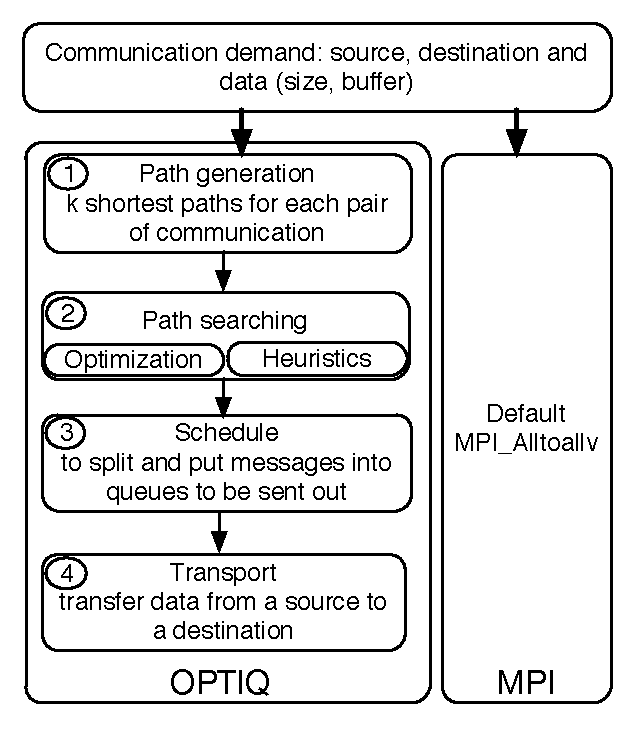
\includegraphics[scale=0.7]{figures/framework.pdf}
\vspace{-0.2in}
\caption{Three components of OPTIQ framework}
\vspace{-0.1in}
\label{fig:framework}
\end{figure}

The functionarity of each component is as following:
\begin{itemize}
\item Path searching: search for path to transfer data from a set of sources to a set of destination. Multiple or single paths can be found using a set of algorithm. User can decide what algorithm to be used or let the framework use a default algorithm.
\item Schedule: Split a buffer data that needed to tranfer into smaller messages and put those messages into a queue of transport layer to be transferred. It also handles incoming messages for itself and for forwardig them to its neighbors on a way to a message final destination.
As we route data in our own ways, we search for the paths, and we also need to schedule messages transfer. It includes sending local messages, forwarding messages form other sources, receiving data as the intermediate node or the destination node.

Order of messages into sending queue: 3 types of messages: local messages (needed to send), fowarding messages (needed to send), its receiving messages. first come first serve, local messages first. forwa

When there are multiple ranks per node, which one will be choosen to receive data at the next dest (forwarding). Single rank to do or many rank to do, currently every rank executes data transfer.

\item Transport: actually transfer an amount of data from one point to another point in the system.
\item Extra component: To get system specific information such as partition size, topology, coordinates, torus, and to compute neighbors of available nodes given to an application. Topology reading, coord, neighbors, torus, size, routing order, graph generated. Also set of benchmarks, tests.

The framework has various options to allow users to tune the framework for optimal performance. For example, the framework allows to select messages from queue to either forward a message from another node first or to send its own message first, to select algorith to search for paths or to set chunk size to transfer a message, to easily add new transport layers on different machine.

\end{itemize}

\section{Benchmarks}
\label{sec:benchmark}

\subsection{Experiment system}
\label{sec:system}

Mira \cite{Chen:BGQ}, with 48 compute racks (48K nodes and 768K cores) at the ALCF, provides 10 PFlops theoretical peak performance. Each node has a 16-core processor and 16 GB of memory.

The interprocess communications of Blue Gene/Q travel on a 5D torus network both for point-to-point and for collective communications. This 5D torus interconnects a compute node with its 10 neighbors at 2 GB/s theoretical peak over each link in each direction, making a total of 40 GB/s bandwidth in both directions for a single compute node. Because of packet and protocol overheads, however, only up to 90\% of the raw data rate (1.8 GB/s) is available for user data. The machine can be partitioned into non-overlapping rectangular submachines; these submachines do not interfere with each other except for I/O nodes and the corresponding storage system.

For interconnect network traffic, BG/Q supports both deterministic and dynamic routing \cite{Chen:BGQ}. In the dynamic routing, messages in different message size ranges can be routed differently. However, within a given message size range, routing is always the same, and its path is known before it is routed. These are the default routing algorithms and cannot be changed during run time. The BG/Q supercomputer uses single-path data routing, for sending/receiving a message only one link of the ten available is used. The details of routing can be found in \cite{Chen:BGQ}.

PAMI is a low-level communication library for BG/Q \cite{PAMI:Kumar}. PAMI provides low-overhead communication by using various techniques such as accelerating communication using threads, scalable atomic primitives, and lockless algorithms to increase the messaging rate. Since MPI is implemented on top of PAMI, direct use of PAMI would provide higher messaging rates as well as lower latencies in comparison with MPI.




\subsection{Synthetic benchmarks}

%We carried our experiments on Mira, a Blue Gene/Q supercomputer. 
We evaluated our approaches on Mira, varying the partition size from 512 nodes to 4096 nodes. %The experiments involved a subset or the entire set of nodes for each partition. 
We varied the number of sources and destinations, and the average distance between them. 
We also experimented with different data sizes to be transferred. 
%We also varied the data sizes to be exchanged to find the effective data size.
We show results for various combinations of source-destination pairs. 
%Pairs of sources and destinations are randomized to show the efficacy of our work. 
The number of shortest paths used by our approaches was 50. % solvers to measure the effectiveness of number of paths to throughput. 
The maximum load $maxload$ for our heuristic approach was 16. 
%A similar benchmark with various max load is done for the heuristic approach. 
%For searching optimal paths we used AMPL (A Modeling Language for Mathematical Programming) and its solvers \cite{AMPL} for modeling our problem, and to find solutions for optimal data movement.


%\subsection{MPI Paths Reconstruction}

In our experiment we need to measure not only the performance of MPI routines, but also loads on physical links, and the number of hops per path that MPI takes to move data from a set of sources to a set of destination. The load and hops informatoon can reveal details on performance differences between MPI and our framework OPTIQ. Thus reconstructing MPI's paths is necessary to get load and hops information.

We reconstruct MPI's paths based on our understanding of default routing algorithms described in \cite{Chen:BGQ}. For each pair of source and destination we start at a source node and follow the rules of the routing algorithm to move data from the source node to its destination. We then record paths for all the pairs and use them to calculate load and number of hops.


\subsection{Communication Patterns}
In this paper we demostrate data movement performance of our OPTIQ framework and existing MPI's routines on the following communication patters:

\begin{figure}[ht]
\vspace{-0.1in}
\centering
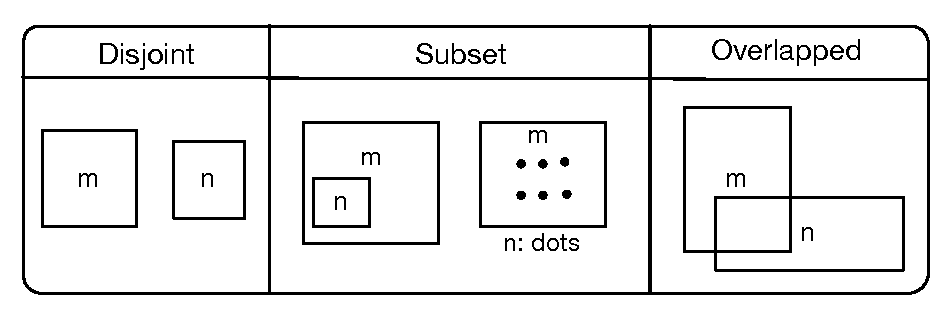
\includegraphics[scale=0.55]{figures/patterns.pdf}
\vspace{-0.1in}
\caption{Communication patterns}
\vspace{-0.1in}
\label{fig:patterns}
\end{figure}

\begin{itemize}
\item Disjoint sets: is many-to-many communication pattern where the sources and destinations are separated. It is a typical pattern in many applications.
\item Overlap: is a many-to-many pattern that sources and destinations are overlapped sets. CESM uses this communication patterns for its coupling communications.
\item Subset: is a many-to-many pattern that sources or destinations are subset of the other. The patterns can be found CESM or in I/O aggregation.
\end{itemize}

We carried a set of experiments to study the system's behavior in various patterns and demontrate throughput improvement.


\subsection{Experiments and Results}

We carried out a set of 91 experiments in which we varied total number of nodes, number of sources, number of destinations, distance between source nodes and destination nodes. We measured the follows: throughput of data transfer, total number of paths found, number of paths per pair of source-destination (a job), hopbytes (multiplication of an amount of data and a number of hops it travels on a path) values on a path, number of paths that shares a physical link, and amount data that passes through a physical link. We used our framework OPTIQ and MPI\_Alltoallv to transfer data and compare 2 ways to show the efficacy of our framework. MPI\_Alltoallv is typical way to transfer data between a set of sources and a set of destinations. It uses default routing algorithms i.e. both dynamic and static routing can be employed. We report some of the resuts in this paper.

\subsubsection{Varying partition, source and destination sizes, keeping the same sources/destination ratio}

\begin{figure*}[!htbp]
        \centering
        \begin{subfigure}[b]{0.32\textwidth}
                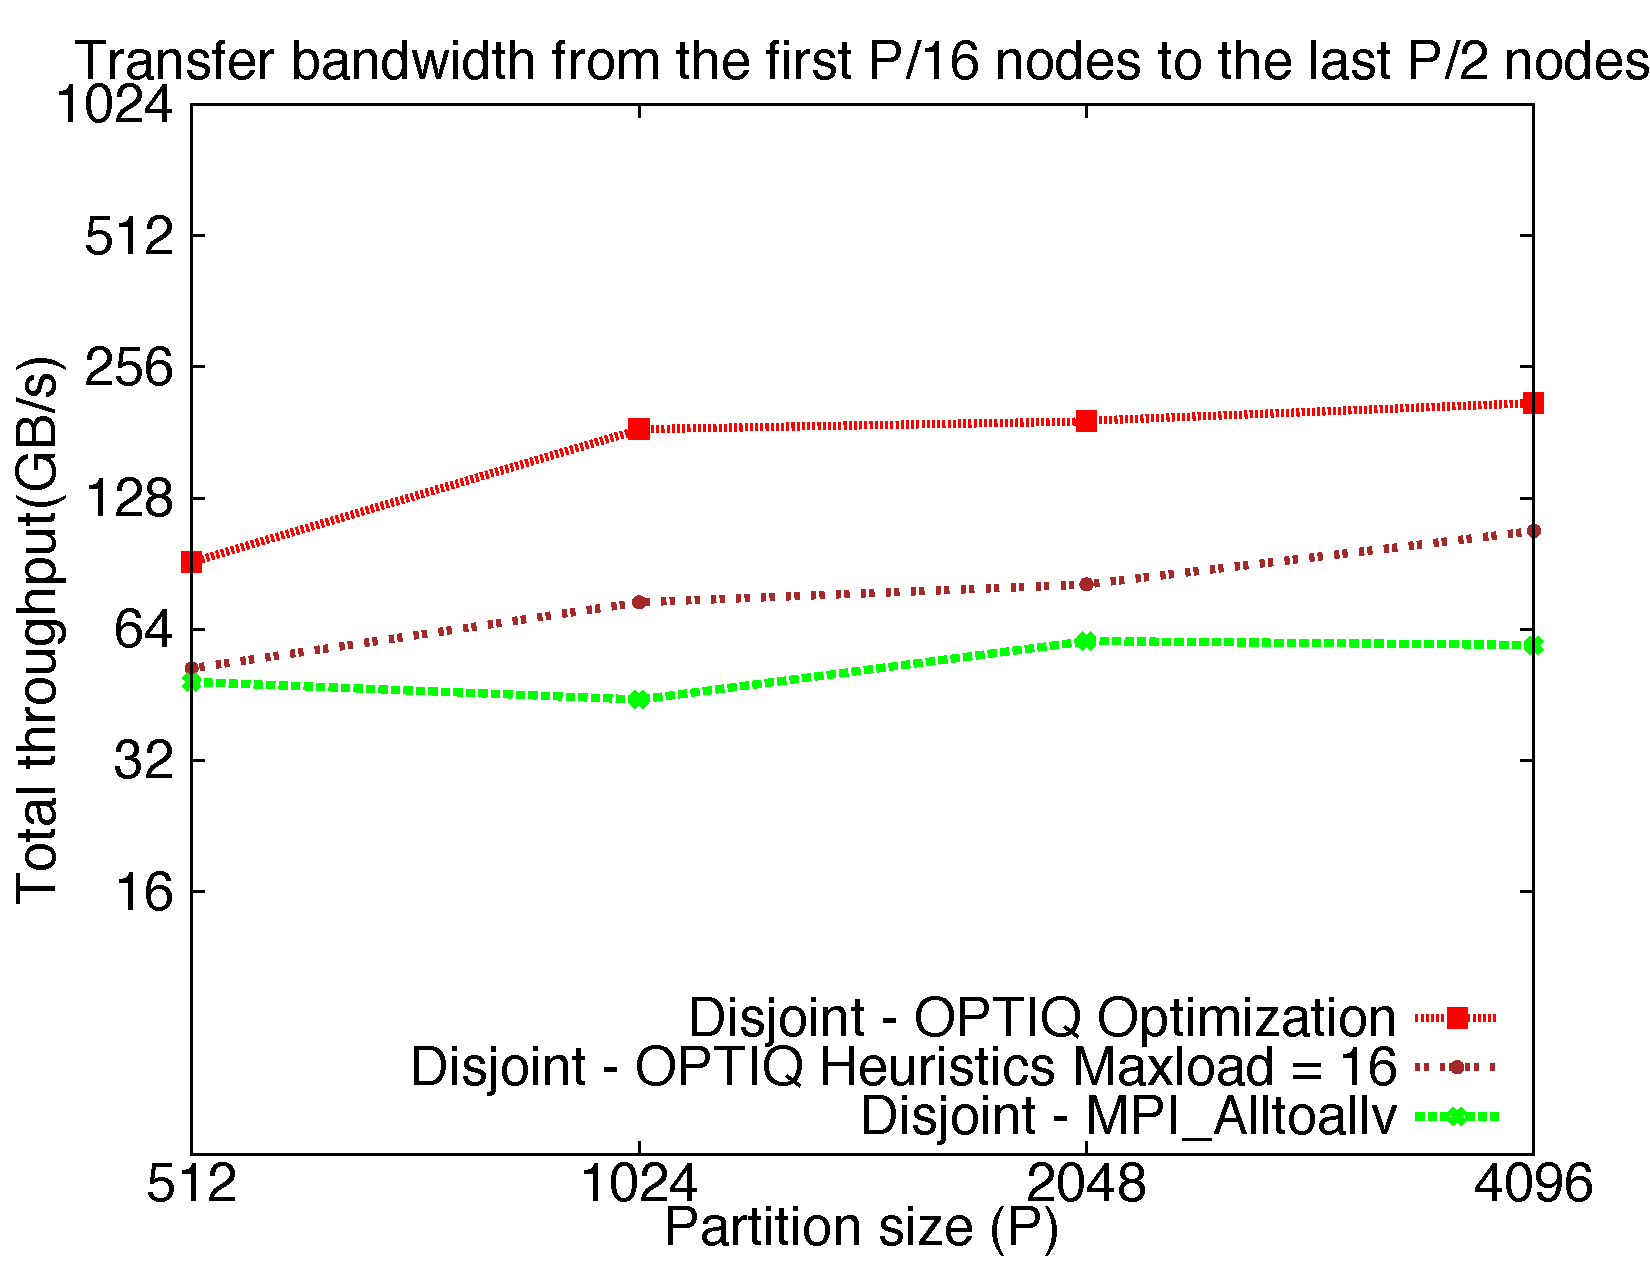
\includegraphics[width=\textwidth]{figures/constantr_3.pdf}
                \caption{Disjoint}
                \label{fig:constantr_3}
        \end{subfigure}%
        ~ %add desired spacing between images, e. g. ~, \quad, \qquad, \hfill etc.
          %(or a blank line to force the subfigure onto a new line)
        \begin{subfigure}[b]{0.32\textwidth}
                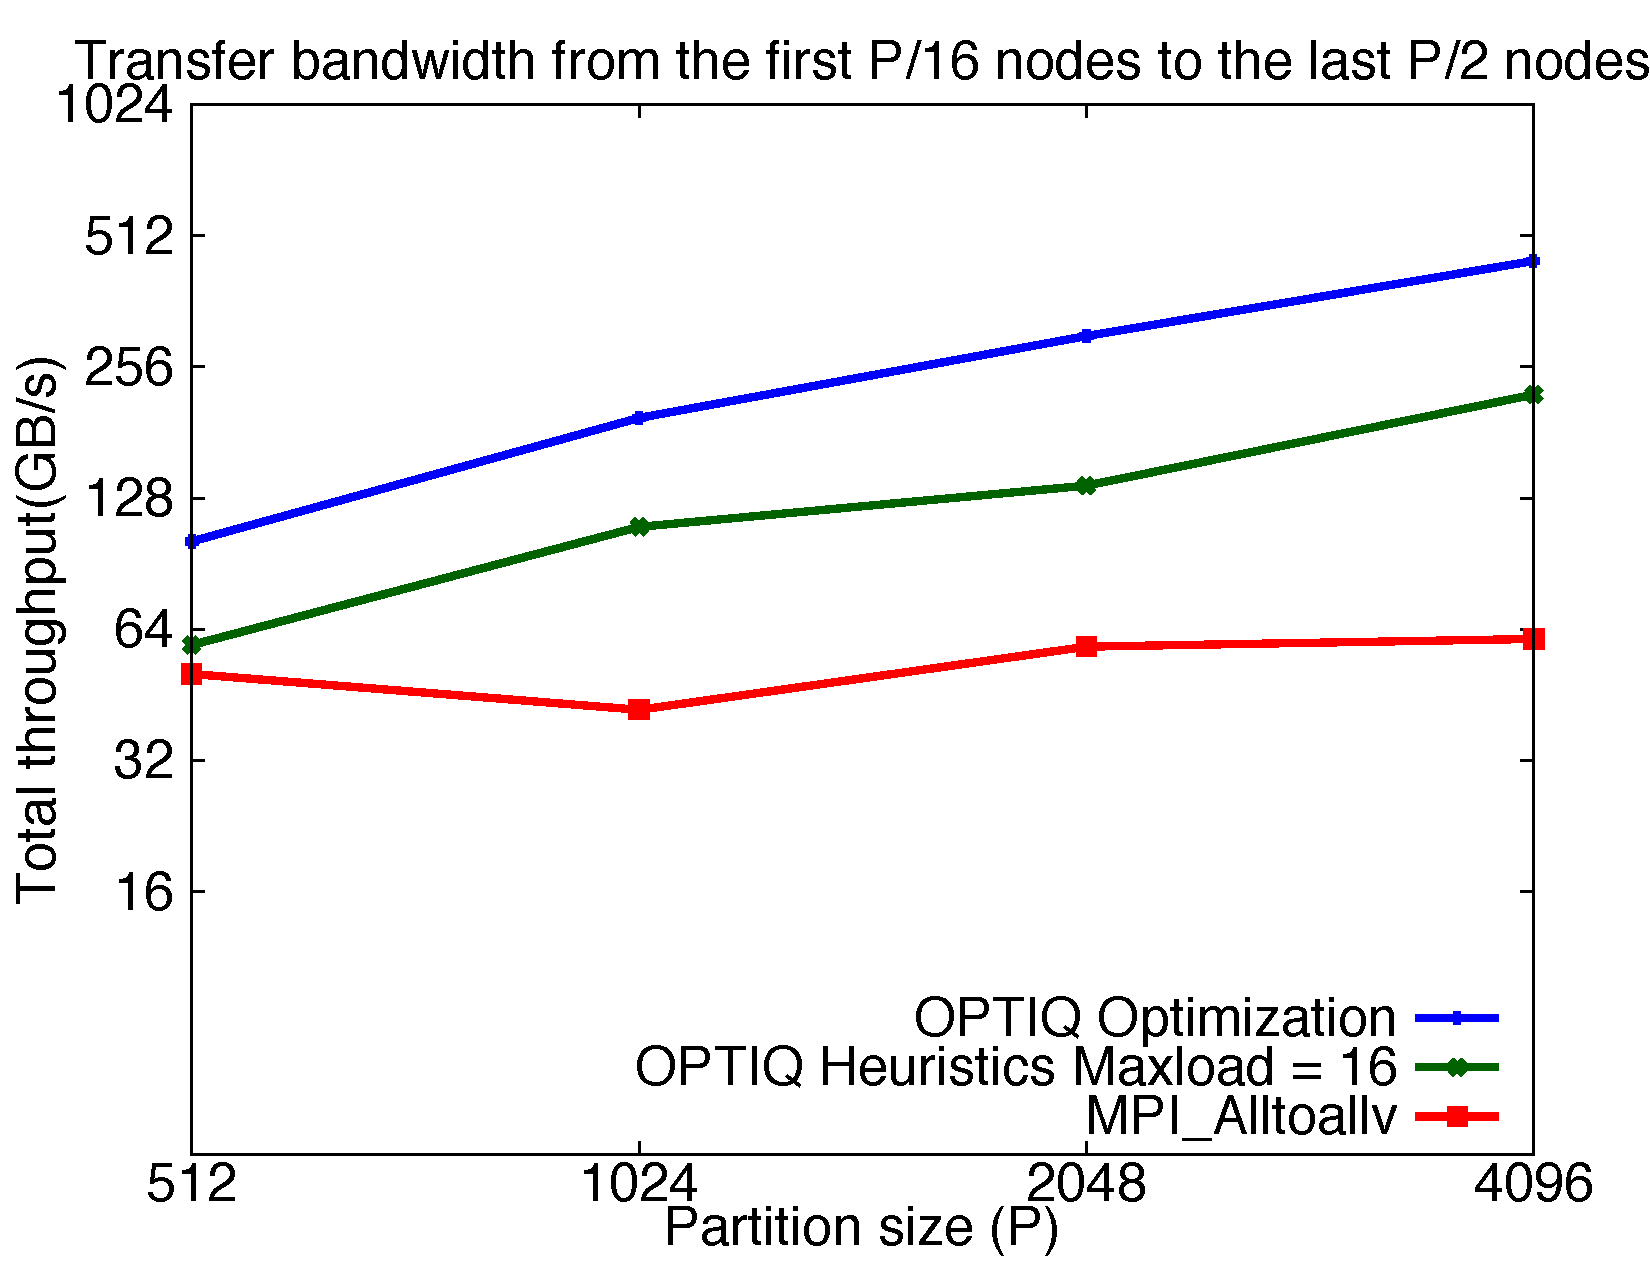
\includegraphics[width=\textwidth]{figures/constantr_27}
                \caption{Overlap}
                \label{fig:constantr_27}
        \end{subfigure}
        ~ %add desired spacing between images, e. g. ~, \quad, \qquad, \hfill etc.
          %(or a blank line to force the subfigure onto a new line)
        \begin{subfigure}[b]{0.32\textwidth}
                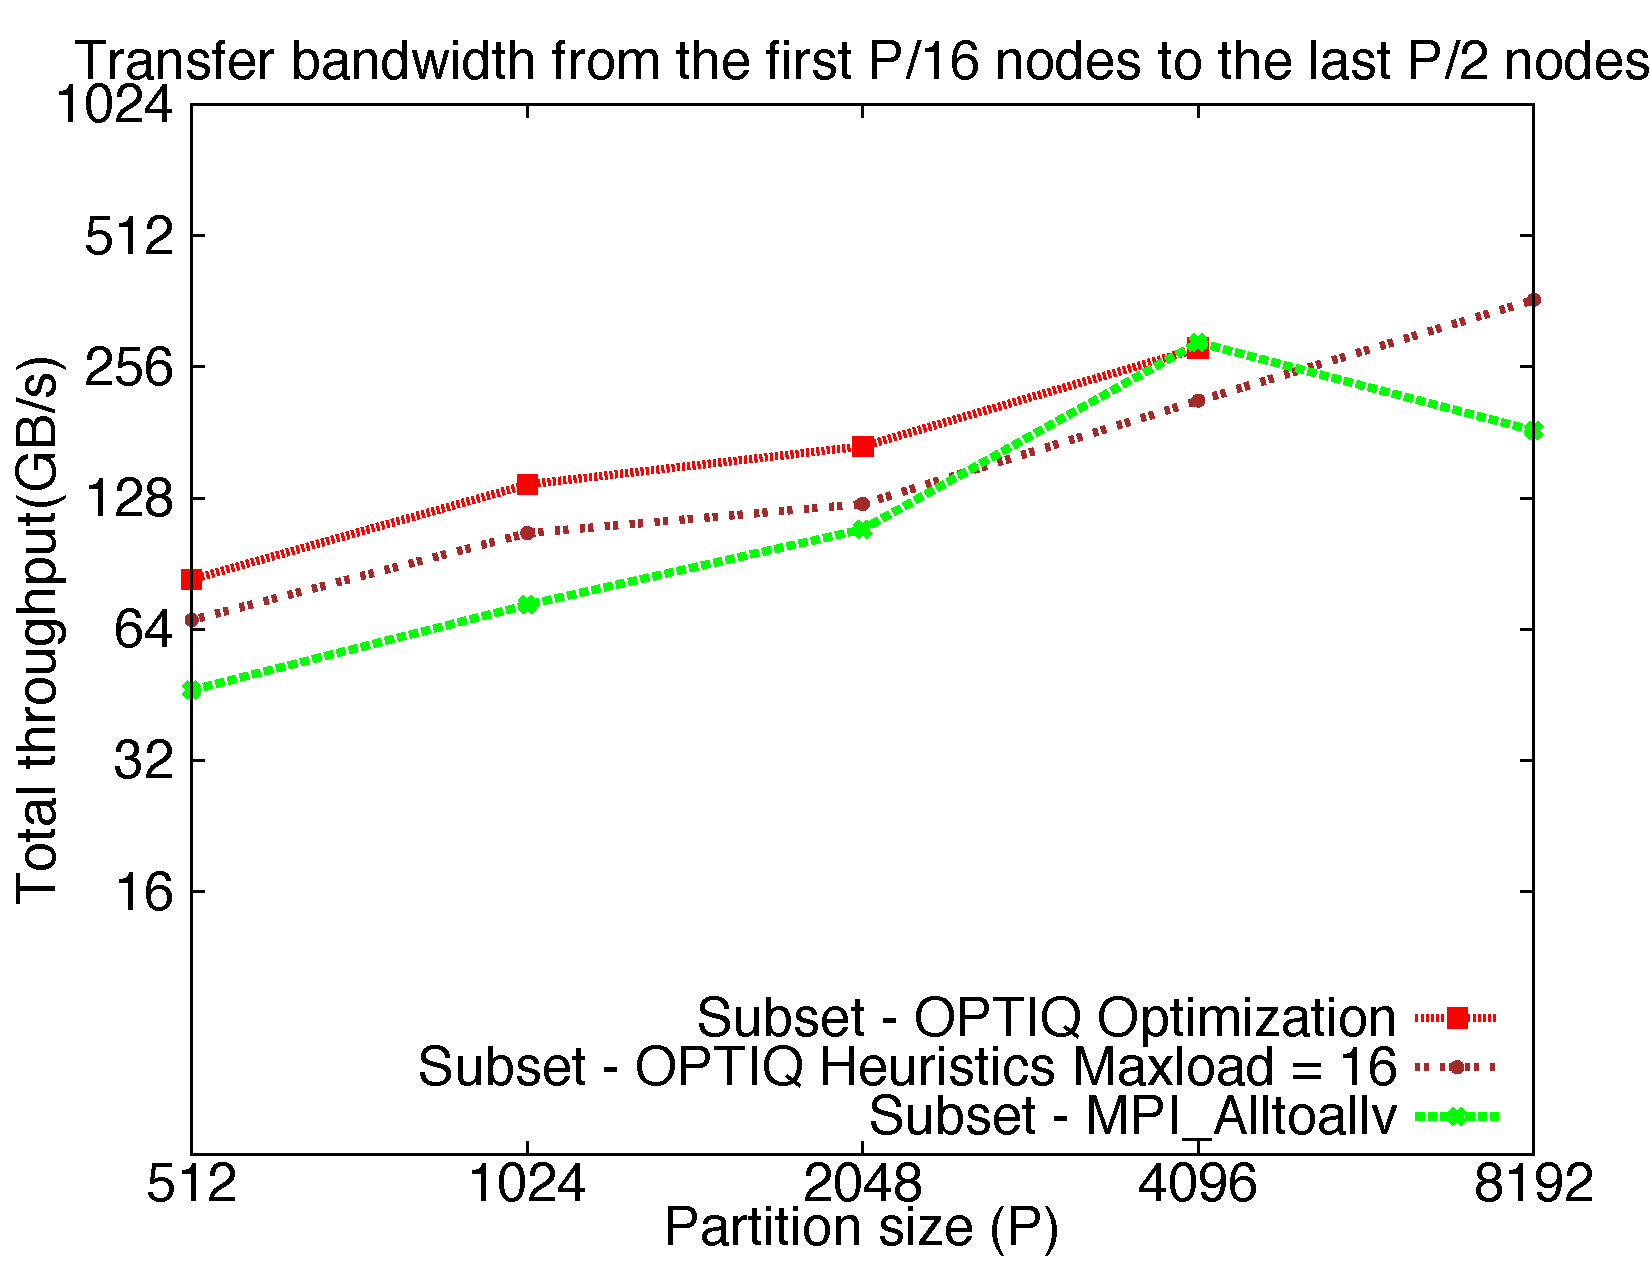
\includegraphics[width=\textwidth]{figures/constantr_87}
                \caption{Subset}
                \label{fig:constantr_87}
        \end{subfigure}
        \caption{Varying the number of sources and destinations and total number of nodes while keeping the ratio constant (1:8).}
        \label{fig:constantr}
\end{figure*}

\begin{table*}[!htbp]
   \centering
    \begin{tabular}{| l | l | r | r | p{0.5cm} | p{0.5cm} | p{0.5cm} | p{0.5cm} |p{0.5cm} | p{0.5cm} |p{0.5cm} | p{0.5cm} |p{0.5cm} | p{0.5cm} |}
    \hline
    \multirow{3}{*}{Pattern} & \multirow{3}{*}{Type} & \multirow{3}{1cm}{BW (GB/s)} & \multicolumn{3}{ c| }{Num. of Paths} & \multicolumn{2}{ c| }{Hopbytes} & \multicolumn{2}{ c| }{Num of copies}& \multicolumn{2}{ c| }{Num of paths} & \multicolumn{2}{ c| }{Total data} \\ \cline{4-6}
    & & & \multirow{2}{0.5cm}{Total Paths} & \multicolumn{2}{ c| }{Per Job} & \multicolumn{2}{ c| }{Per Path (MB)} & \multicolumn{2}{ c| }{Per Path}& \multicolumn{2}{ c| }{Per Link}& \multicolumn{2}{ c| }{Per Link (MB)} \\ \cline{5-14}
    & & & & {Max} & Avg & Max & Avg & Max & Avg & Max & Avg & Max & Avg\\ \hline
    \multirow{3}{*}{Disjont} & OPT    & 188.62 & 1,169 & 6 & 2.28 & 83.88 & 23.02 & 1152 & 295.22 & 11 & 2.53 & 18.28 & 9.26 \\ \cline{2-14}
    & HEU & 74.88  & 3,146 & 23 & 6.14 & 83.88 & 8.45 & 1152 & 108.24 & 16 & 4.94 & 63.04 & 6.92 \\ \cline{2-14}
    & MPI    & 45.18  & 512  & 1 & 1.00 & 92.27 & 50.33 & & & 16 & 3.07 & 134.21 & 25.76\\ \hline
    \multirow{3}{*}{Overlap} & OPT    & 200.03 & 1303 & 6 & 2.54 & 83.88 & 19.28  & 1152 & 243.96 & 13 & 2.74 & 16.97 & 9.04\\ \cline{2-14}
    & HEU & 113.17  & 3273 & 26 & 6.39 & 75.49 & 7.41 & 1024 & 93.07 & 16 & 5.17 & 38.66 & 7.04 \\ \cline{2-14}
    & MPI    & 42.84 & 512 & 1 & 1.00 & 83.88 & 42.99 &  & & 16 & 3.38 & 134.21 & 28.36 \\ \hline
    \multirow{3}{*}{Subset} & OPT    & 199.20 & 1269 & 6 & 2.48 & 75.49 & 19.48 & 1024 & 245.66 & 11 & 2.79 & 17.10 & 9.32 \\ \cline{2-14}
    & HEU &  61.71 & 3238 & 26 & 6.32 & 75.49 & 7.43 & 1024 & 93.22 & 16 & 5.28 & 45.08  & 7.35 \\ \cline{2-14}
    & MPI    &  41.37 & 512  & 1 & 1.00 & 83.88 &  41.94 & & & 16 & 3.52 & 134.21 & 29.49 \\ \hline
    \end{tabular}
    \caption{Throughput, total num of paths, number of paths per job, maximum and average values of hopbytes, number of copies, number of paths per link and amount of data per link for 3 patterns in 1024 nodes experiments.}
    \label{table:constantr}
\end{table*}

\begin{figure}[!htb]
\vspace{-0.1in}
\centering
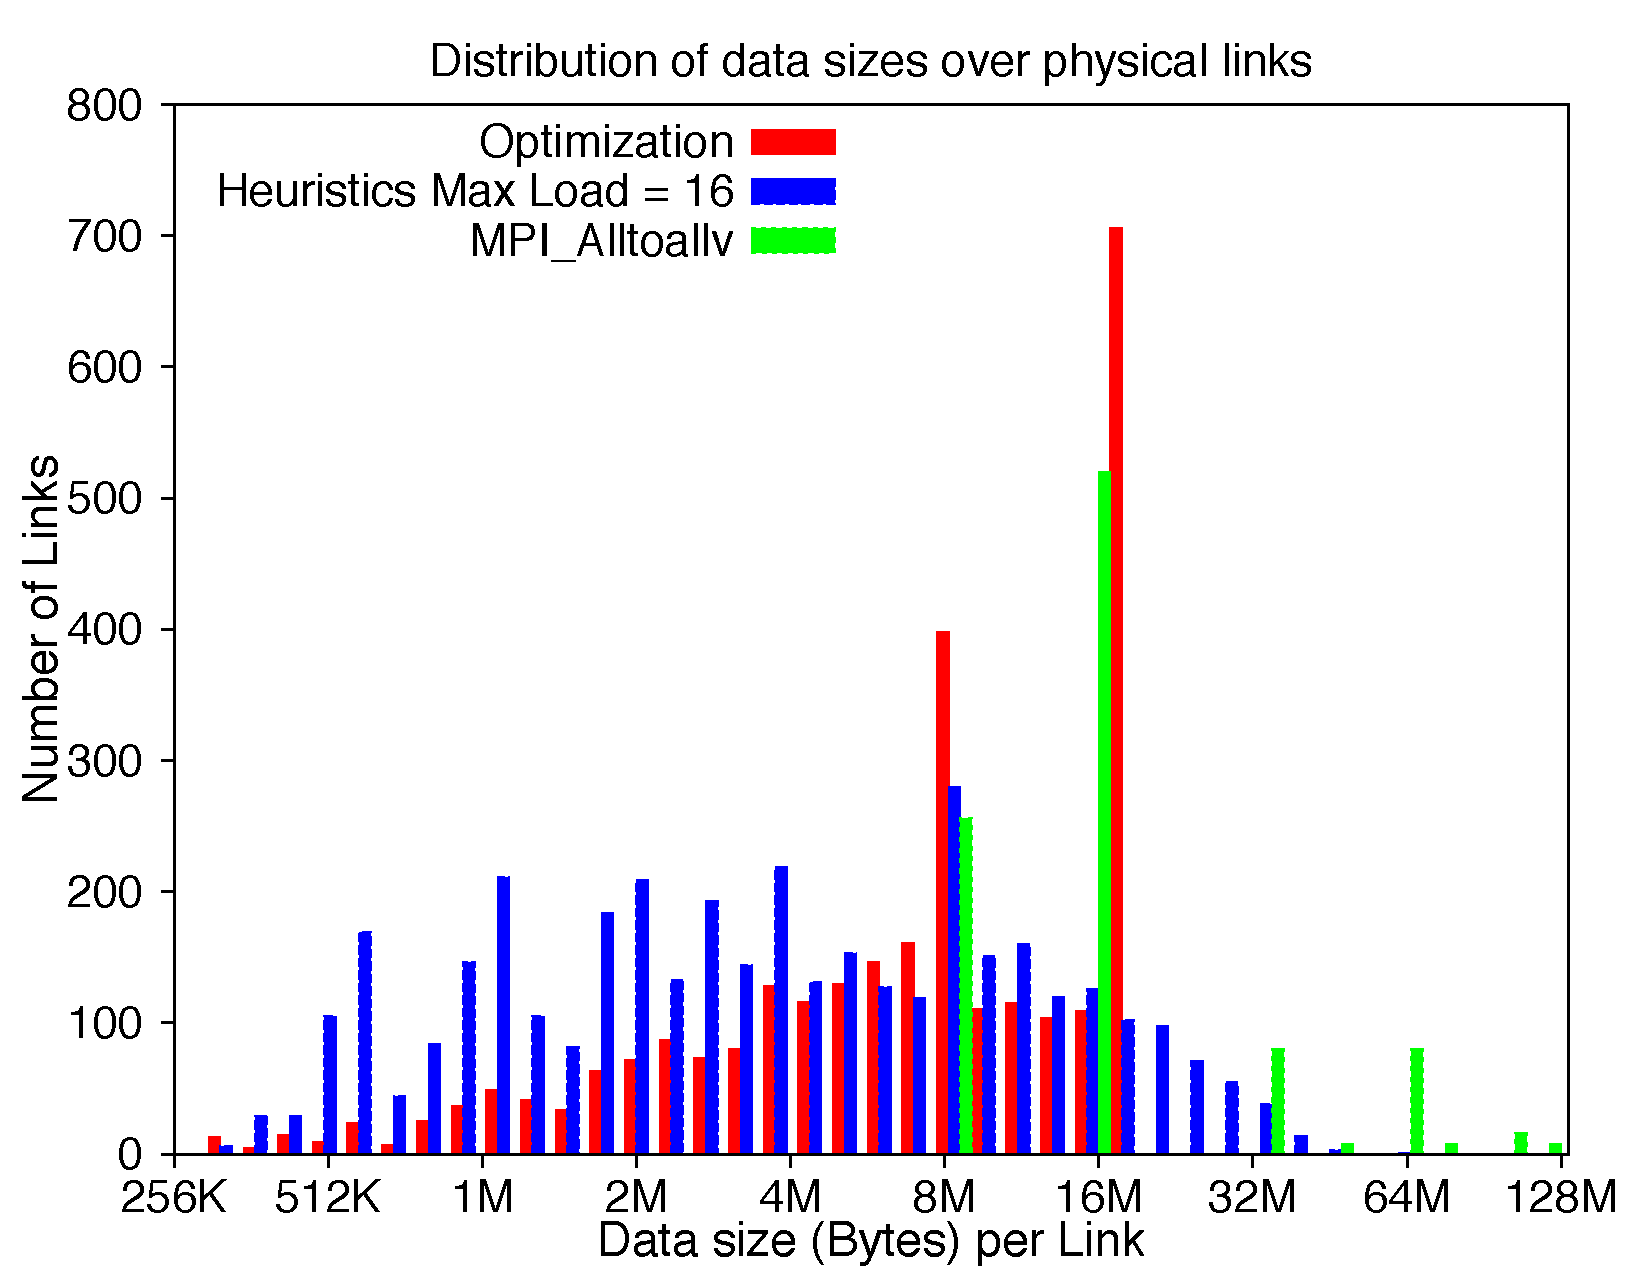
\includegraphics[scale=0.30]{figures/loaddata_histo.pdf}
\vspace{-0.1in}
\caption{Distribution of total amount of data per link for Disjoint pattern in 1024-node partition.}
\vspace{-0.1in}
\label{fig:loaddata_histo}
\end{figure}

\begin{figure}[!htb]
\vspace{-0.1in}
\centering
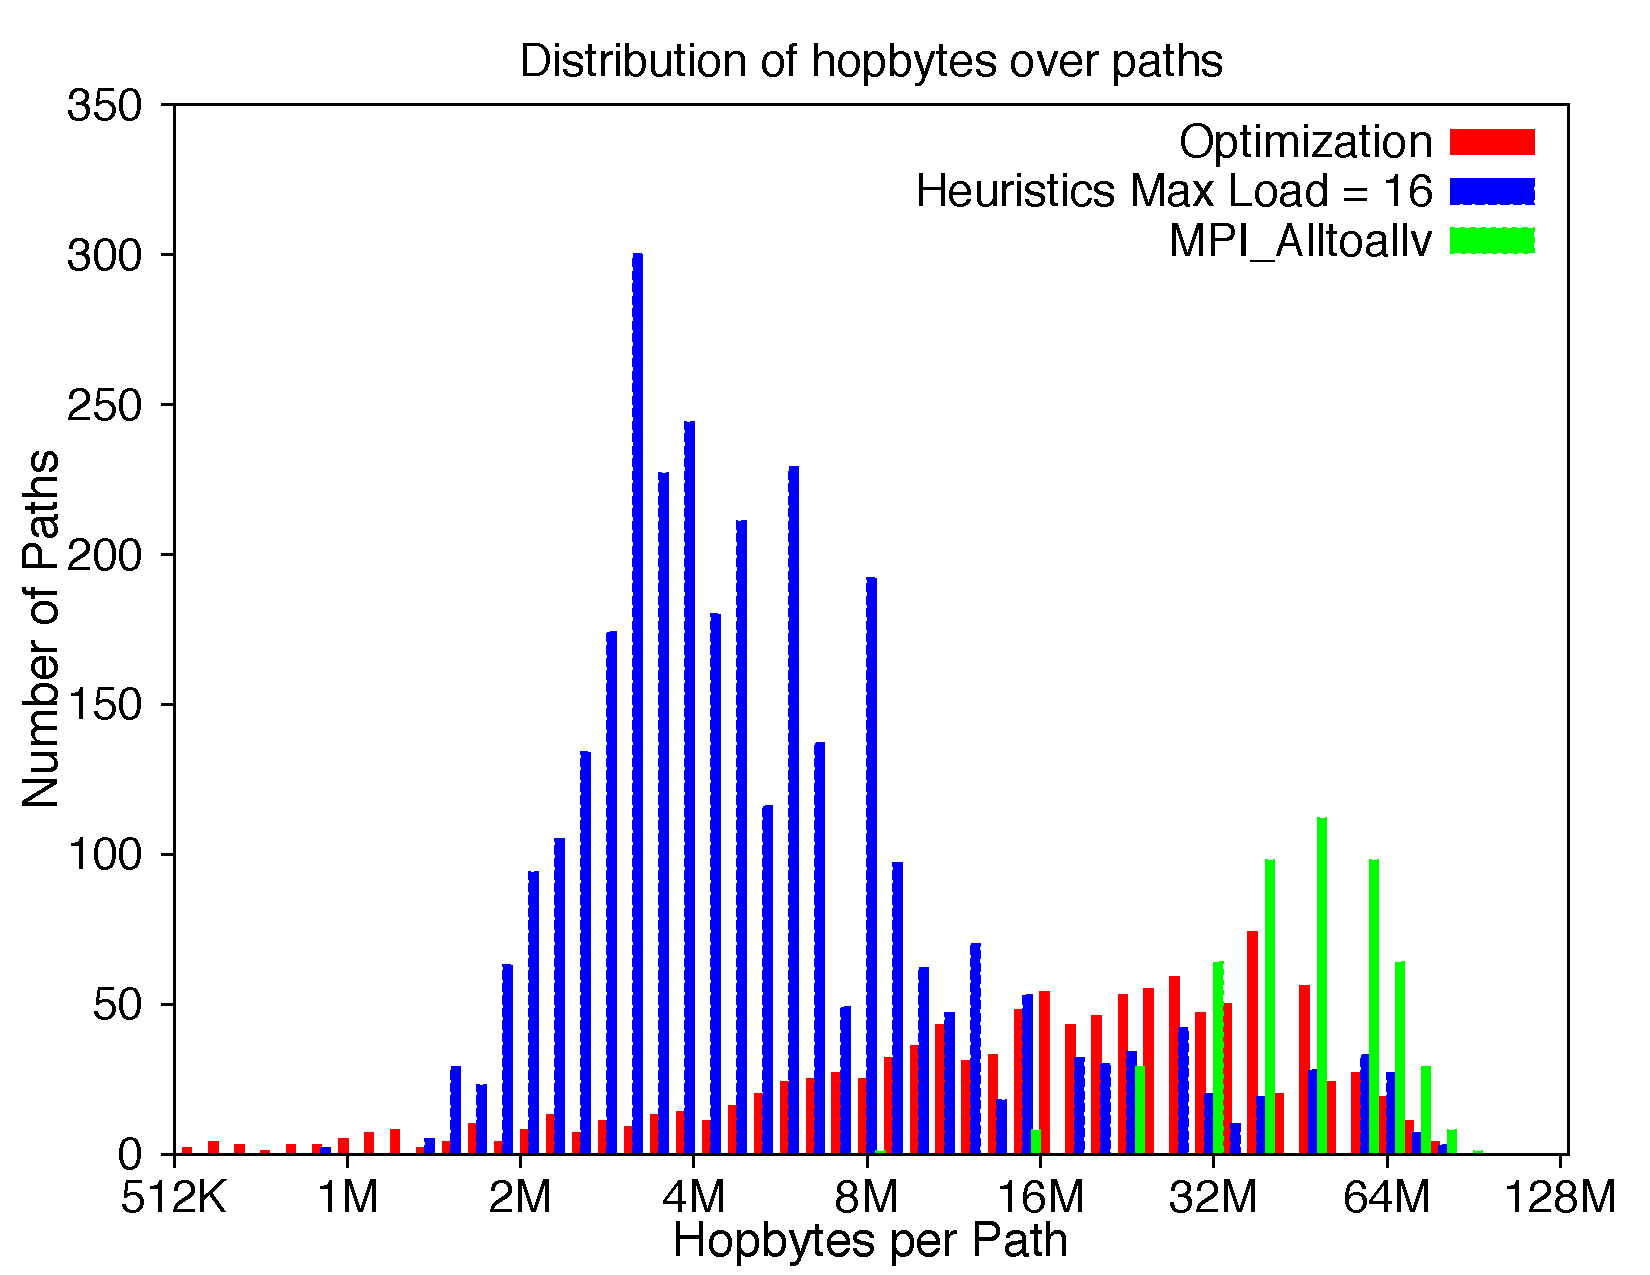
\includegraphics[scale=0.30]{figures/hopbyte_histo.pdf}
\vspace{-0.1in}
\caption{Distribution of hopbytes per path for Disjoint pattern in 1024-node partition.}
\vspace{-0.1in}
\label{fig:hopbyte_histo}
\end{figure}

In this experiment we vary the number of sources and destinations together with total number of nodes while keeping the ratio between the number of sources and destination at 1/8. While the total number of nodes P  increases from 512 to 4096 the first P/16 nodes send data to the last P/2 nodes. Each source has 8 destinations e.g node 0 sends data to nodes P/2, P/2+1, ...P/2+7. We tested the framework for 3 patterns: subset, disjoint and overlap, with 3 approaches of transferring data OPTIQ Optimization, OPTIQ Heuristics and MPI\_Alltoallv. We use 1 MPI/PAMI rank/node. The data size is 8 MB per pair. We set the $maxload$ to 16 for the Heuristic approach.

As shown in Figure \ref{fig:constantr} the Optimization approach has the highest throughput, the Heuristics approach is next and MPI\_Alltoall achieved the lowest throughput. The Table \ref{table:constantr} shows that in all three patterns the Heuristic with $maxload$ set to 16 was able to find highest number of paths. The Heurisc approach also has the highest maximum and average number paths for a job. As data is divided equally among paths, this led to lowest maximum and average values for hopbytes, number of copies per path. However this led to higher number of paths per physical link, and higher amount of data per physical link in the Heuristic approach in comparison to the Optimization approach. In Optimization the data is split among the paths to balance the amount of data between physical links, thus it has the lowest maximum amount of data per physical link. The distribution of the total amount of data in Figure \ref{fig:loaddata_histo} also shows this effect. This led to its highest throughput. MPI\_Alltoall approach has the lowest number of paths. With 1 path per pair of communication, data is not split. Thus it has the the highest hopbytes per path and amount of data per physical link. The distribution of its total data size per link in Figure \ref{fig:loaddata_histo} and its hopbytes per paths in Figure \ref{fig:hopbyte_histo} also show the effects. Both factors led to its lowest throughput.


\subsubsection {Three communication patterns with random message sizes}
In this experiment, we varied the number of source nodes, number of destination nodes and total number of nodes (partition sizes) but kept the ratio between the source nodes and the destination nodes constant. With P is size of the partition, we choose the first P/16 nodes as the source nodes, and N/2 last nodes as the destination nodes. Each node in the set of source nodes communicates with 8 nodes in the set of destination nodes. The pairing is aligned i.e. node 0 communicates with nodes (P/2, ..., P/2/7). We randomly choosing the data size for each pair of communication from 64 KB up to 8 MB of data. We experimented with 3 communication patterns: Disjoint, Overlap, Subset and 3 approaches: Optimization, Heuristic and MPI\_Alltoallv. We used only 1 MPI/PAMI rank per node. The total number of nodes P varied from 512 up to 4096 nodes. The communication throughputs are shown in Figure \ref{fig:constantr_msg}.

\begin{figure*}[!htbp]
        \centering
        \begin{subfigure}[b]{0.32\textwidth}
                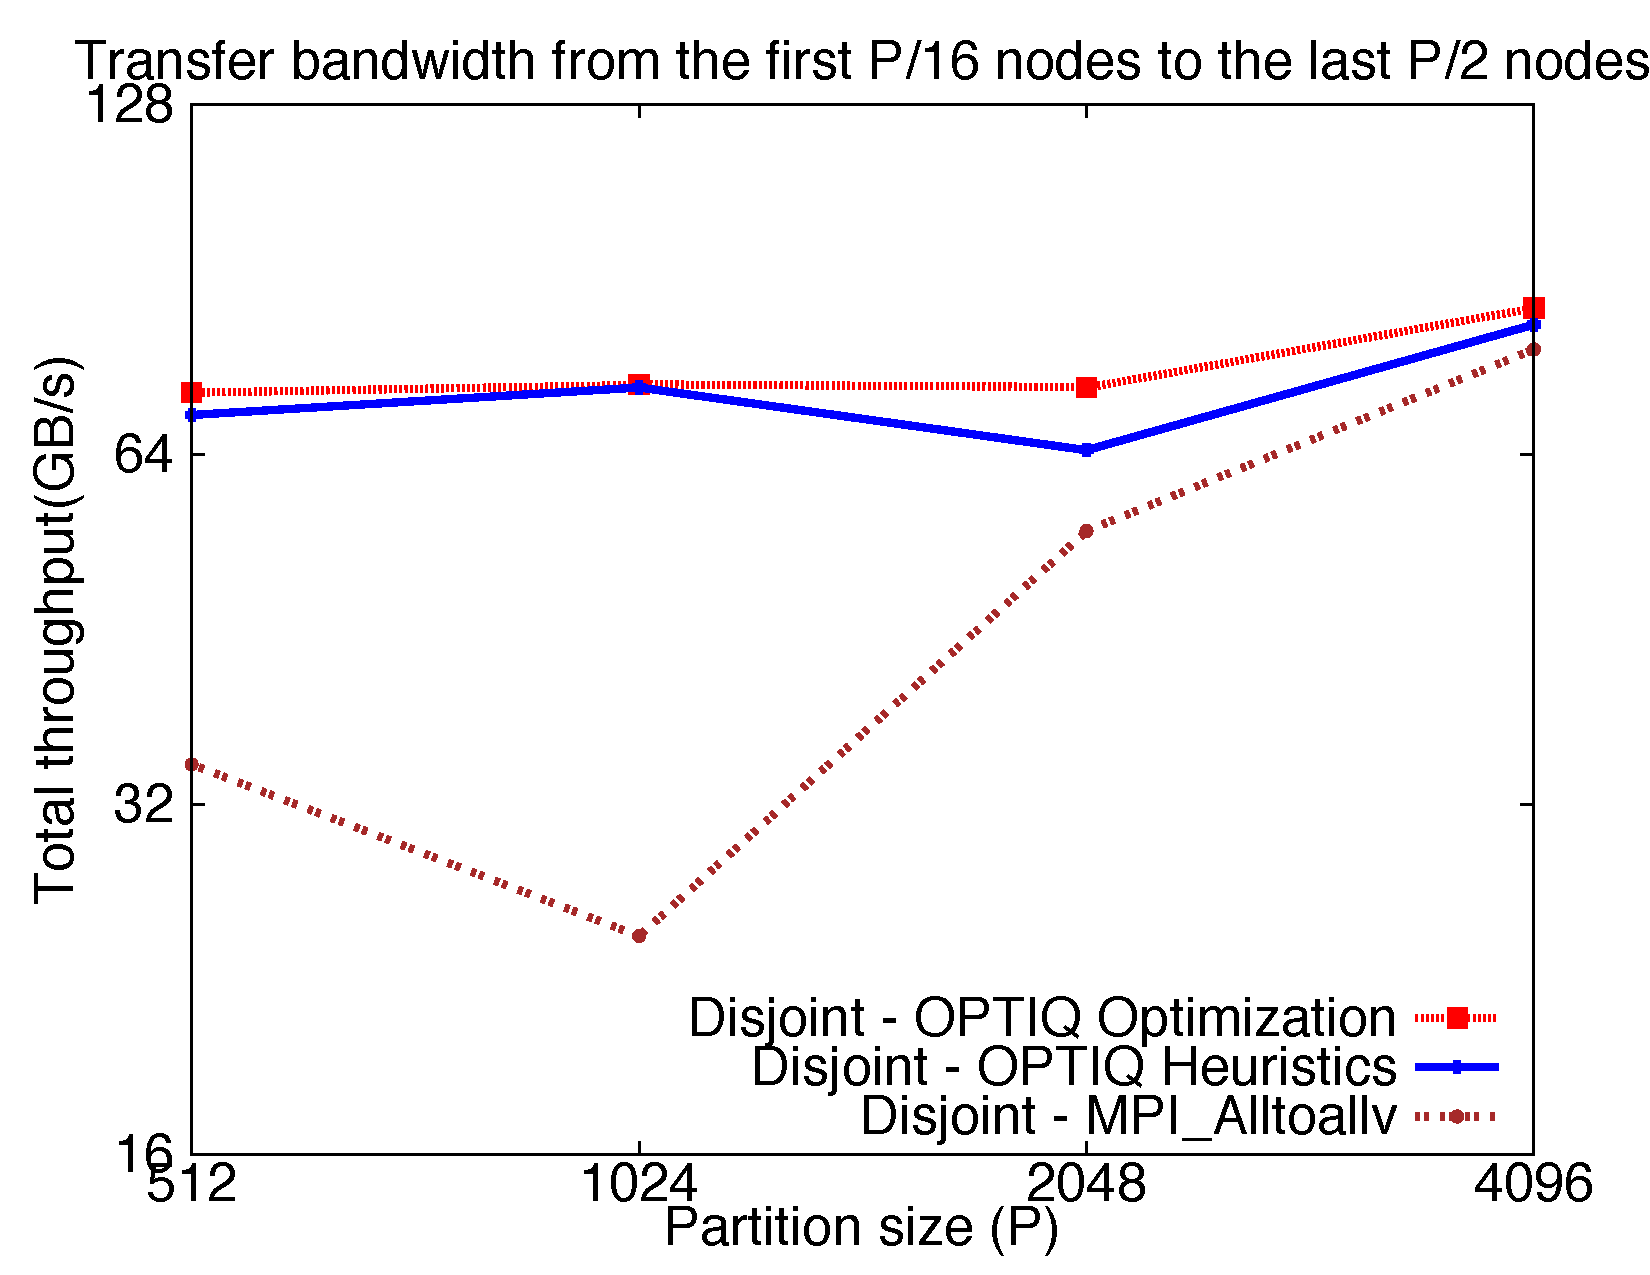
\includegraphics[width=\textwidth]{figures/constantr_disjoint_msg.pdf}
                \caption{Disjoint}
                \label{fig:constantr_disjoint_msg}
        \end{subfigure}%
        ~ %add desired spacing between images, e. g. ~, \quad, \qquad, \hfill etc.
          %(or a blank line to force the subfigure onto a new line)
        \begin{subfigure}[b]{0.32\textwidth}
                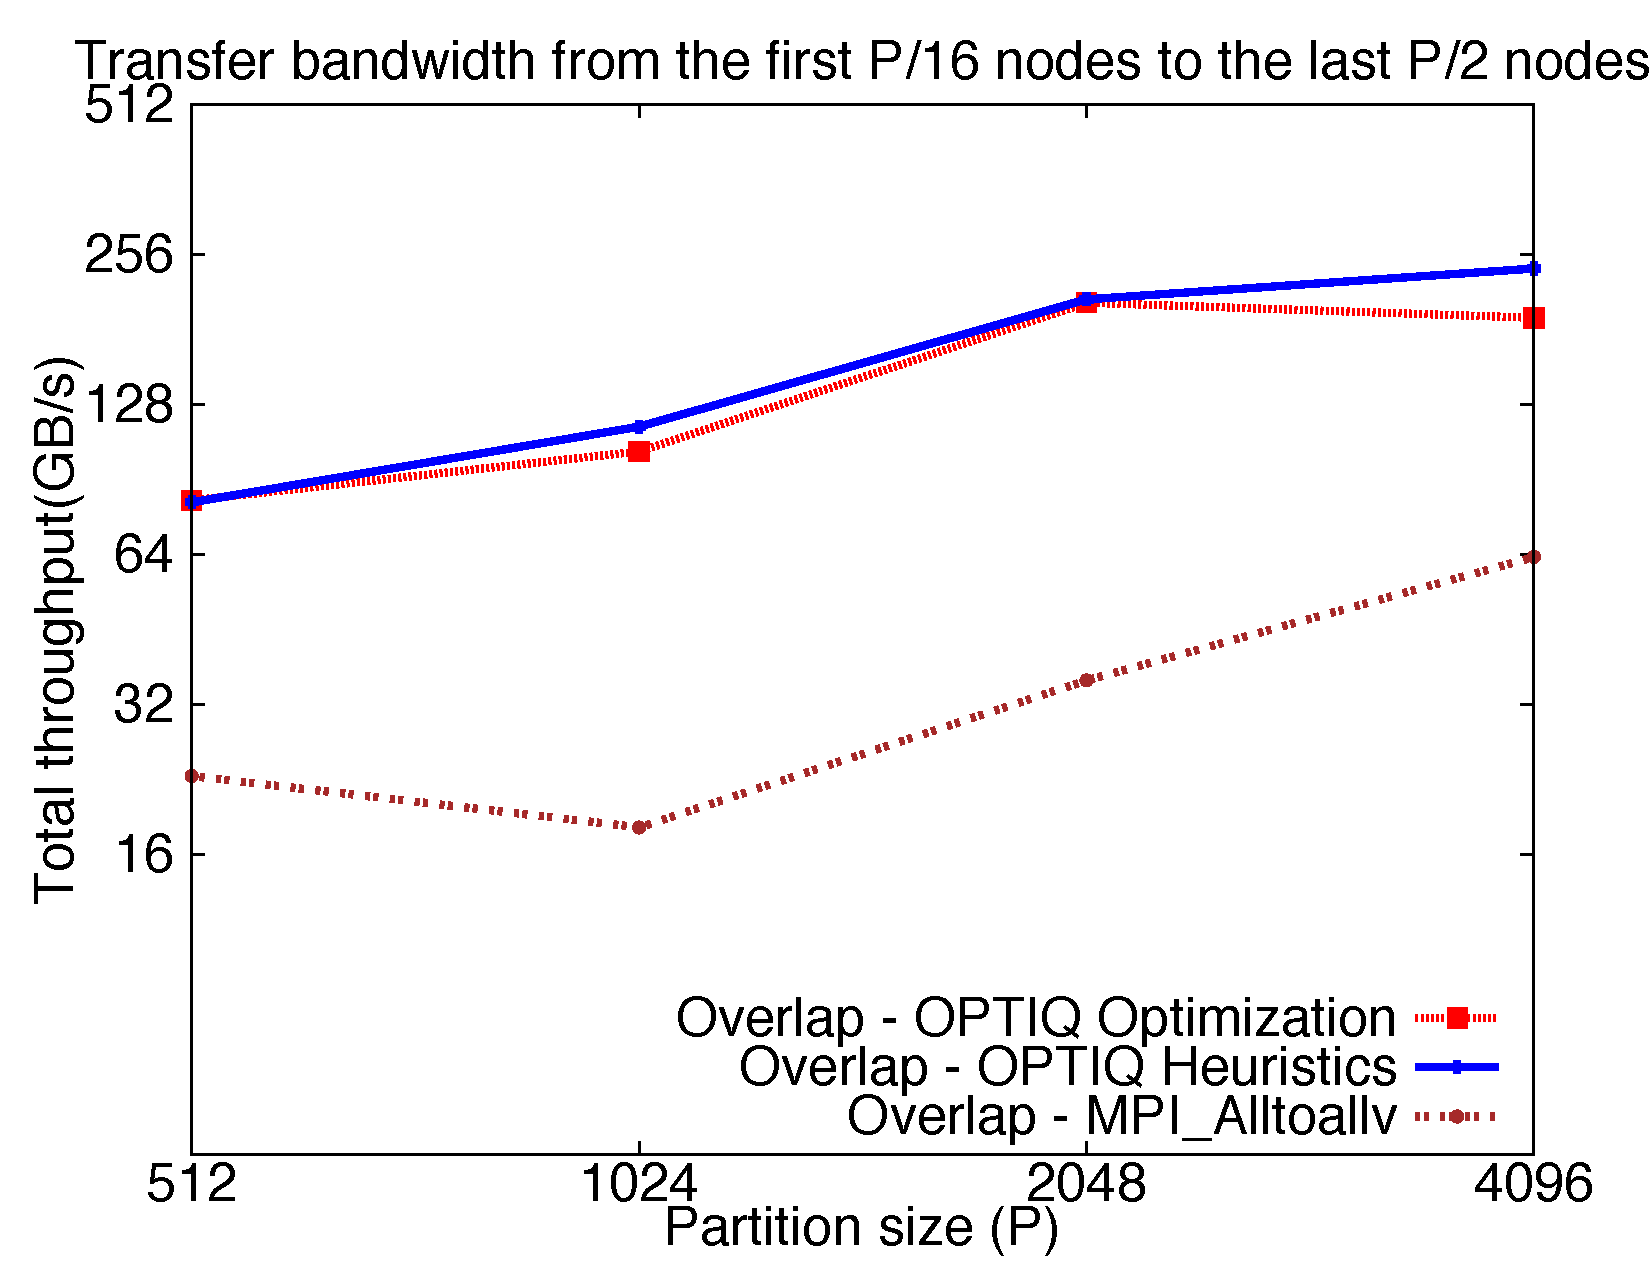
\includegraphics[width=\textwidth]{figures/constantr_overlap_msg.pdf}
                \caption{Overlap}
                \label{fig:constantr_overlap_msg}
        \end{subfigure}
        ~ %add desired spacing between images, e. g. ~, \quad, \qquad, \hfill etc.
          %(or a blank line to force the subfigure onto a new line)
        \begin{subfigure}[b]{0.32\textwidth}
                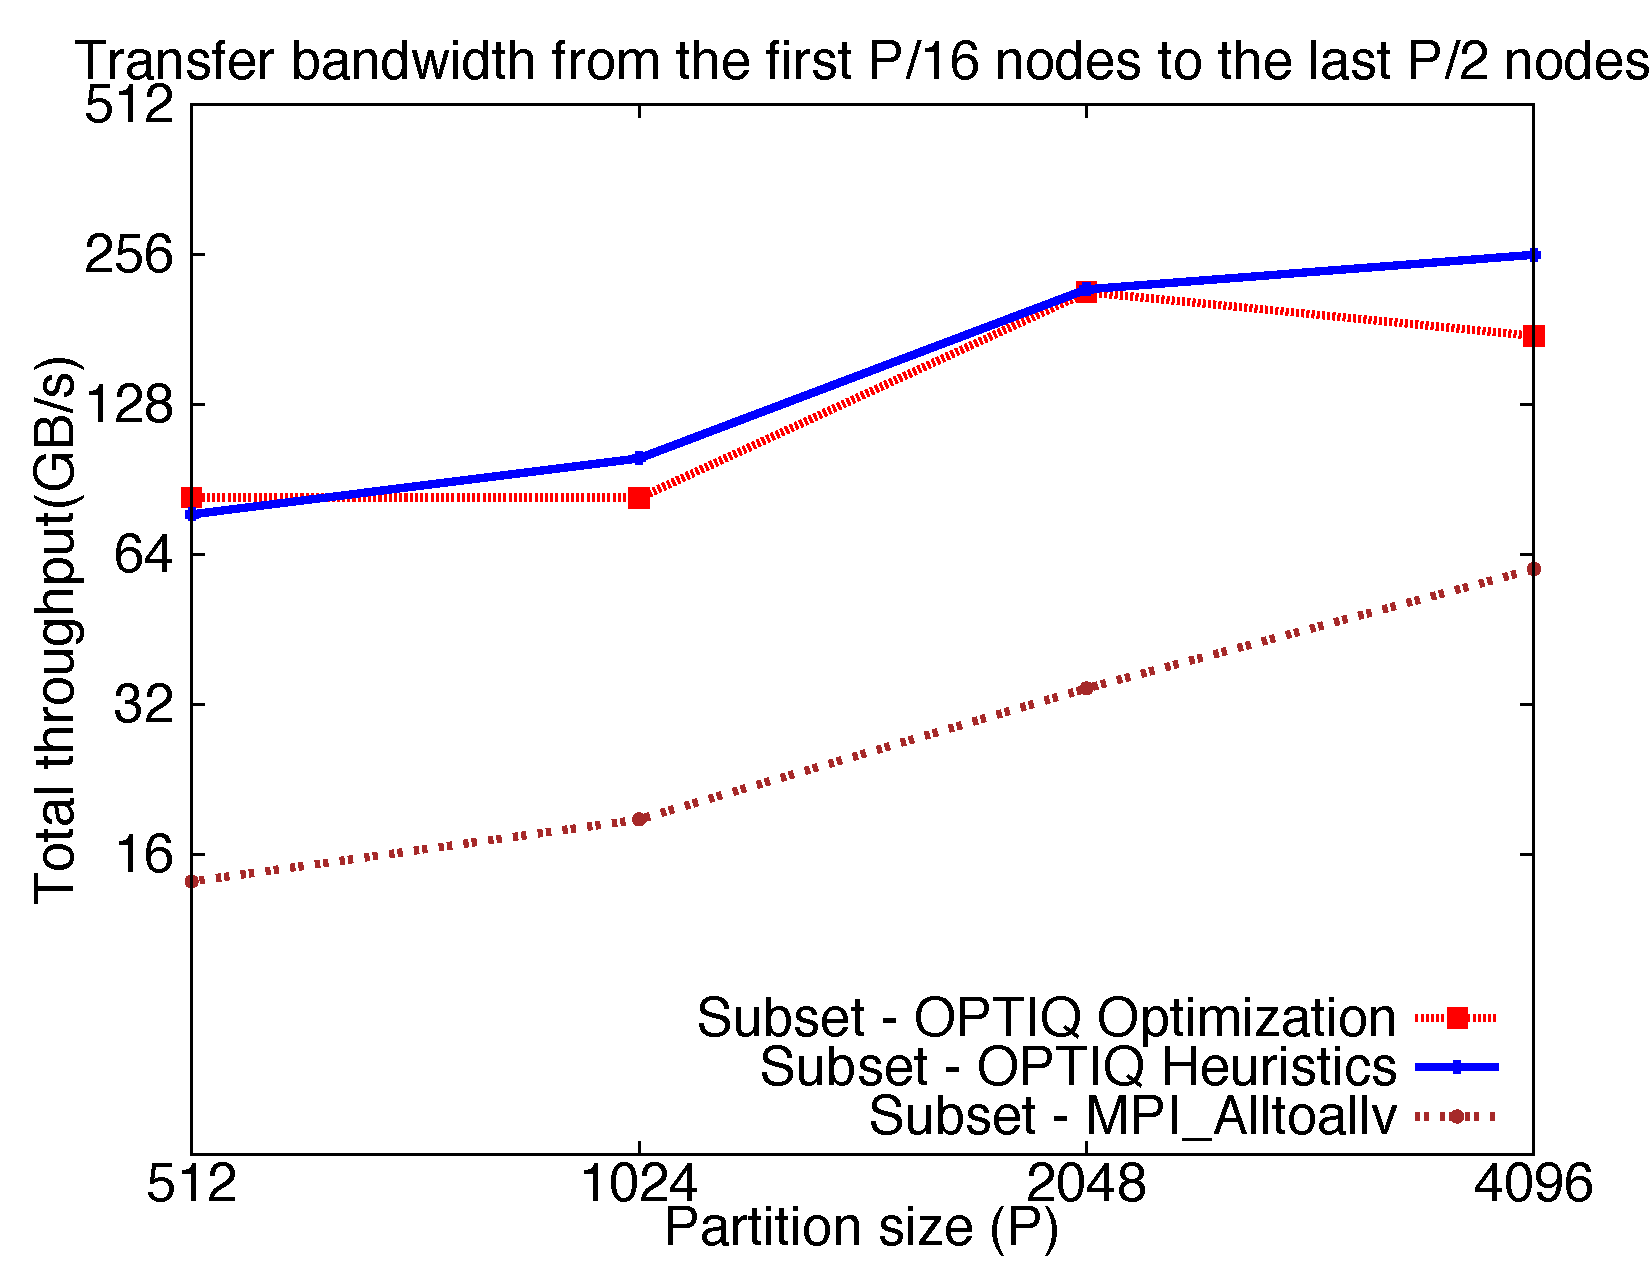
\includegraphics[width=\textwidth]{figures/constantr_subset_msg.pdf}
                \caption{Subset}
                \label{fig:constantr_subset_msg}
        \end{subfigure}
        \caption{Varying the number of sources and destinations and total number of nodes with constant ratio}
        \label{fig:constantr_msg}
\end{figure*}

As shown in the Figure \ref{fig:constantr_msg}, in all the three communication patterns, Optimization approach and Heuristic approach have similar performance and is both significant higher than MPI\_Alltoallv in most of the experiments. In Disjoint pattern, the performance gap is close at 4096 nodes with at the other 2 patterns, the gap is quite constant showing the scalability of our approaches.

In the next section, we demonstrate the efficacy of our approaches through an experiment with communication patterns and data from a real application Community Earth System Model (CESM).


%\subsubsection {Multiple ranks}
%In this experiment, we demonstrate the scalability of our framework when increasing the number of MPI/PAMI ranks per node.


\section{Conclusion}
\label{sec:conclusion}
%In this paper 
We proposed two approaches for balancing load on the Blue Gene/Q supercomputer using multiple paths for data movement. We realized our approaches in OPTIQ framework and demonstrated the efficacy of our work through a set of benchmarks. Overall, we improved throughput by 43\%--67\% on average for three different communication patterns in 91 experiments on up to 4096 nodes. %Performance, however, can be improved up to 4X. %what does this mean? 
Our work shows that to improve data movement performance we need to take advantage of both application's data movement patterns and system routing algorithms. In general, our Optimization approach outperforms heuristic and MPI\_Alltoallv due to better load-balanced multiple paths for data movement. In future, we plan to study these approaches on the Cray XE6 supercomputer and test them with real applications.


% conference papers do not normally have an appendix


% use section* for acknowledgement
\section*{Acknowledgment}


The authors would like to thank...
more thanks here


% trigger a \newpage just before the given reference
% number - used to balance the columns on the last page
% adjust value as needed - may need to be readjusted if
% the document is modified later
%\IEEEtriggeratref{8}
% The "triggered" command can be changed if desired:
%\IEEEtriggercmd{\enlargethispage{-5in}}

% references section

% can use a bibliography generated by BibTeX as a .bbl file
% BibTeX documentation can be easily obtained at:
% http://www.ctan.org/tex-archive/biblio/bibtex/contrib/doc/
% The IEEEtran BibTeX style support page is at:
% http://www.michaelshell.org/tex/ieeetran/bibtex/
\bibliographystyle{IEEEtran}
% argument is your BibTeX string definitions and bibliography database(s)
\bibliography{IEEEabrv,thesis.bib}
%
% <OR> manually copy in the resultant .bbl file
% set second argument of \begin to the number of references
% (used to reserve space for the reference number labels box)
%\begin{thebibliography}{1}

%\bibitem{IEEEhowto:kopka}
%H.~Kopka and P.~W. Daly, \emph{A Guide to \LaTeX}, 3rd~ed.\hskip 1em plus
%  0.5em minus 0.4em\relax Harlow, England: Addison-Wesley, 1999.

%\end{thebibliography}




% that's all folks
\end{document}


